\apendice{Especificación de diseño}

\section{Introducción}

En este anexo se introducirá el diseño de los distintos aspectos de este proyecto a todos los niveles \textit{software}.

\section{Diseño de datos}

En este trabajo se manejan dos tipos de datos principales:

\begin{itemize}
	\item Imágenes con formato JPG.
	\item Ficheros JSON que contienen las coordenadas de las etiquetas realizadas con el etiquetador de imágenes.
\end{itemize}

Tanto las imágenes como las etiquetas de las imágenes se almacenan de manera persistente en nuestro disco duro. Para observarlas, deberemos navegar, dentro del proyecto, por la siguiente ruta de carpetas: \textit{code}, \textit{rsc}, \textit{img}. Una vez situados en la carpeta \textit{img}, nos encontraremos una serie de carpetas con el nombre de cada tipo de fitolito y una carpeta \textit{Default}\footnote{Siempre y cuando hayamos utilizado el etiquetador anteriormente.}.

La razón de la existencia de una carpeta por cada tipo de fitolito es el almacenamiento organizado de los recortes generados por el etiquetador. Almacenando en cada una de estas carpetas los recortes o imágenes correspondientes a un tipo de fitolito. 

Respecto a la carpeta \textit{Default}, en ella se almacenan las imágenes completas junto a un fichero \textit{JSON} por imagen. En cada uno de estos ficheros se almacenan las coordenadas  realizadas con el etiquetador en dicha imagen. Un ejemplo del contenido de un fichero JSON sería el mostrado en la figura \ref{fig:C.1.1}.

\begin{figure}
\centering
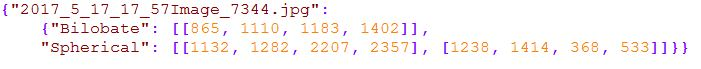
\includegraphics[width=0.9\textwidth]{json_example}
\caption{Ejemplo de fichero JSON.}
\label{fig:C.1.1}
\end{figure}

Siendo el formato: nombre de la imagen y nombre de cada tipo de fitolito, solo apareciendo los existentes en la imagen. Teniendo cada tipo de fitolito una lista de etiquetas, donde cada etiqueta tiene cuatro coordenadas. Las cuatro coordenadas se almacenan con el siguiente orden y significado:

\begin{itemize}
	\item Desplazamiento en el eje y de la esquina superior izquierda de una etiqueta.
	\item  Desplazamiento en el eje y de la esquina inferior derecha de una etiqueta.
	\item Desplazamiento en el eje x de la esquina superior izquierda de una etiqueta.
	\item  Desplazamiento en el eje x de la esquina inferior derecha de una etiqueta.
\end{itemize}
%Captura

\section{Diseño procedimental}

En este proyecto hay que destacar tres procedimientos principales, los cuales explicaré, brevemente, a continuación.

\begin{comment}
\begin{itemize}
	\item Procedimiento que realiza el etiquetador de imágenes.
	\item Procedimiento en el \textit{notebook} para la detección de caras.
	\item Procedimiento de entrenamiento de \textit{YOLO}.
\end{itemize}
\end{comment}

\subsection{Procedimiento que realiza el etiquetador de imágenes}

El procedimiento muy simplificado del funcionamiento del etiquetador cuando se carga una nueva imagen es el mostrado en el procedimiento \ref{alg:1}.

\begin{algorithm}
    \If{Cambio de imagen}
    	{
    	Cargamos imagen.
    	
    	\If{La imagen se encuentra en el directorio por defecto y tiene un fichero JSON correspondiente}
    		{
    			Cargamos las etiquetas previamente realizadas.
    			
    			Mostramos las etiquetas junto a la imagen.
    		}
    	Escuchamos los eventos del ratón sobre el SVG.
    	}
    \caption{Procedimiento de funcionamiento del etiquetador}
    \label{alg:1}
\end{algorithm}

Una vez cargada la imagen, como indico finalmente, se escuchan los eventos del ratón. En concreto, los \textit{clicks} y movimientos de este sobre el SVG. Ya que la creación de los rectangulos, o etiquetas, sobre la imagen se hacen a partir de dichos eventos. Para ello, se poseen dos \textit{listeners}, u observadores de eventos, uno para cada evento. Los \textit{clicks} se utilizan para la creación de un nuevo rectángulo o su finalización. Y los movimientos del ratón, una vez hecho un primer click\footnote{De manera que hayamos creado el rectángulo.}, permiten redimensionar el rectángulo de manera totalmente intuitiva.

Nótese que existen más variables a tener en cuenta, como el tipo de fitolito, el cual determina el directorio donde se guardará el recorte obtenido de la etiqueta y como se almacenan las coordenadas en el fichero \textit{JSON}, entre otras. Pero lo que se intenta realizar en este apartado es una explicación simplificada del procedimiento.

\subsection{Procedimiento en el \textit{notebook} para la detección de caras}

El procedimiento simplificado del funcionamiento del \textit{notebook} para el reconocimiento de caras en una imagen es el mostrado en el procedimiento~\ref{alg:2}.

\begin{algorithm}
    Realizamos la ventana deslizante sobre la imagen.    
    
    \ForEach{ventana}{%
    Obtenemos las características del histograma de los gradientes.

	Clasificamos la imagen.    
    }
    
    Eliminamos las ventanas redundantes con non-maximum suppression.

    Mostramos la imagen con los rectángulos.
    \caption{Procedimiento de funcionamiento del etiquetador}
    \label{alg:2}
\end{algorithm}

\subsection{Procedimiento para la detección de fitolitos}

El procedimiento del funcionamiento del \textit{notebook} para el reconocimiento de fitolitos en una imagen es muy similar al mostrado en~\ref{alg:2}. El procedimiento es el mostrado en~\ref{alg:3}.

\begin{algorithm}
    Realizamos la ventana deslizante sobre la imagen.    
    
    \ForEach{ventana}{%
    Obtenemos las características.
    
    Realizamos agrupamiento sobre las características.
    
    Obtenemos histograma.    
    
    Clasificamos la imagen. 
    }	   
    
    Eliminamos las ventanas redundantes con non-maximum suppression.

    Mostramos la imagen con los rectángulos.
    \caption{Procedimiento de reconocimiento de fitolitos}
    \label{alg:3}
\end{algorithm}

\section{Diseño arquitectónico}

En este apartado se representan los aspectos más relevantes a nivel de diseño arquitectónico mediante la notación UML.

Este proyecto no contiene un diseño muy elaborado a nivel arquitectónico por dos razones fundamentales. La primera ha sido el esfuerzo requerido en la investigación y el aprendizaje de técnicas muy variadas para afrontar el problema. Hasta dar con la más adecuada. Por otro lado, la mayoría del código ha sido desarrollado en los \textit{Jupyter Notebooks}. Los cuales nos permiten interaccionar fácilmente con el código y documentarlo a su vez, aportando una fácil introducción a otros usuarios.

Aun así existen tres módulos con código empaquetado: módulo utilizado para la gestión de carpetas del etiquetador, módulo utilizado para la predicción de caras y el modulo para la predicción de fitolitos. Véase el diagrama de paquetes \ref{fig:C.4.1}.

\begin{figure}
\centering
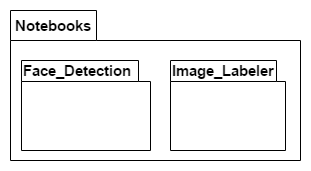
\includegraphics[width=0.4\textwidth]{dia_paquetes}
\caption{Diagrama de paquetes}
\label{fig:C.4.1}
\end{figure}

\subsection{Modulo para la gestión de carpetas}

Por un lado, tenemos el módulo que se encarga de la gestión de carpetas donde el etiquetador almacena las imágenes. Véase el diagrama de clases \ref{fig:C.4.2}.

\begin{figure}
\centering
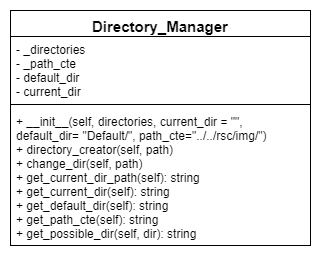
\includegraphics[width=0.4\textwidth]{dia_dirs}
\caption{Diagrama de la clase encargada de la gestión de carpetas}
\label{fig:C.4.2}
\end{figure}

\subsection{Modulo para la predicción de caras}

Por otro lado, tenemos las clases encargadas de la predicción de caras en una nueva imagen mediante el \textit{notebook} explicado anteriormente. En este caso existen 3 clases, las cuales interaccionan entre sí. La primera es una clase estática con 2 funciones para los cálculos del non-maximum suppression y la ventana deslizante. Véase la figura \ref{fig:C.4.3} 


\begin{figure}
\centering
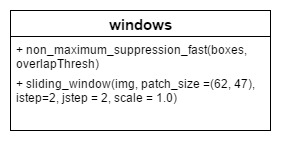
\includegraphics[width=0.4\textwidth]{dia_win}
\caption[Clase estática encargada de varias tareas]{Clase estática encargada de las tareas de non-maximum suppression y ventana deslizante}
\label{fig:C.4.3}
\end{figure}

Además, tenemos la clase encargada de envolver al clasificador y realizar las tareas de clasificación de una imagen. Véase la figura \ref{fig:C.4.4}. Y, finalmente, tenemos la clase encargada de guardar la imagen, mostrarla y poder clasificarla con el apoyo del resto de clases. Véase la figura \ref{fig:C.4.5}. Para finalizar este modulo, podemos apreciar en la figura \ref{fig:C.4.6} como interaccionan las tres clases.

\begin{figure}
\centering
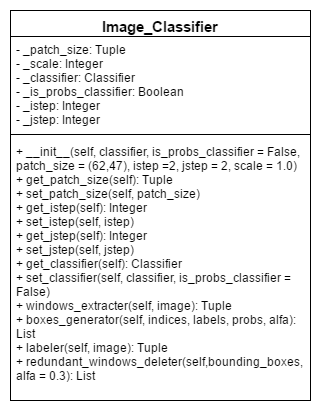
\includegraphics[width=0.4\textwidth]{dia_ic}
\caption{Clase encargada de las tareas de clasificación de una imagen}
\label{fig:C.4.4}
\end{figure}

\begin{figure}
\centering
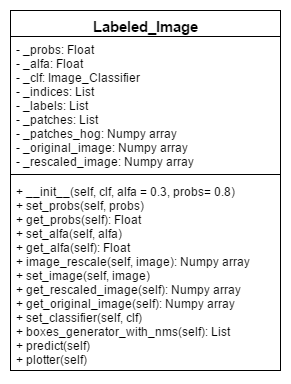
\includegraphics[width=0.4\textwidth]{dia_li}
\caption[Clases encargadas de la clasificación]{Clase encargada de de guardar la imagen, mostrarla y poder clasificarla.}
\label{fig:C.4.5}
\end{figure}

\begin{figure}
\centering
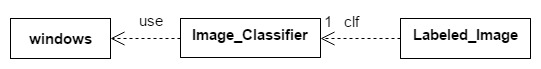
\includegraphics[width=0.99\textwidth]{dia_cls}
\caption{Diagrama de clases del \textit{Jupyter Notebook} para la detección de caras.}
\label{fig:C.4.6}
\end{figure}

\subsection{Modulo para la predicción de fitolitos}

Por último, el modulo más importante que consta de unicamente 2 clases: la clase encargada de la clasificación de fitolitos y la clase encargada de el reconocimiento de objetos en imágenes de fitolitos, representadas en la figura~\ref{fig:C.4.7}.

\begin{figure}
\centering
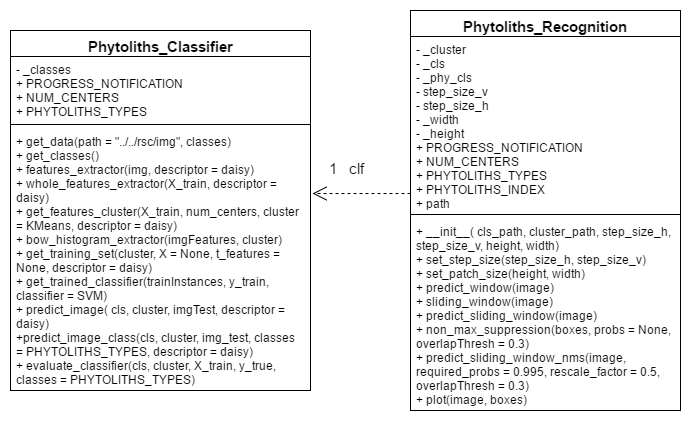
\includegraphics[width=0.99\textwidth]{dia_phy}
\caption{Diagrama de clases para la detección de fitolitos.}
\label{fig:C.4.7}
\end{figure}

\section{Diseño de las interfaces}

En esta sección se explicarán las diferentes interfaces de los productos realizados en este trabajo fin de grado.

\subsection{\textit{Jupyter Notebook} para la detección de caras}

Durante el primer mes se trabajó en un \textit{Jupyter Notebook} que trataba de reconocer caras mediante un clasificador junto a un extractor de características, como ya hemos explicado en secciones anteriores. Con este \textit{Jupyter Notebook} se trataba de facilitar la evaluación del rendimiento de los clasificadores y el cambio de las distintas variables de manera interactiva. 

Por lo tanto, la interfaz de este \textit{Jupyter Notebook} no ha sido trabajada para su uso por parte del usuario. Sino que fue creada para un uso más de experimentación. Es por ello que la interfaz no tiene un buen grado de usabilidad como podemos observar en la figura \ref{fig:C.5.1}.

\begin{figure}
\centering
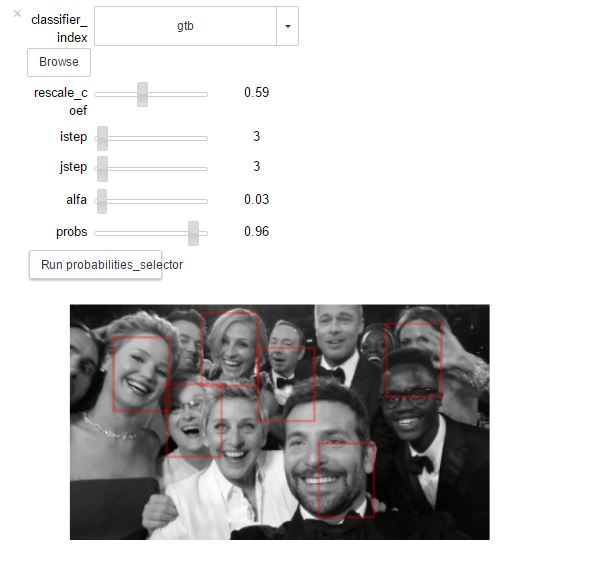
\includegraphics[width=0.99\textwidth]{reconocimiento_de_caras_notebook_v1}
\caption{\textit{Jupyter Notebook} para el reconomiento de caras}
\label{fig:C.5.1}
\end{figure}

\begin{comment}
\begin{itemize}
	\item \textit{classifier_index}: permite seleccionar el clasificador con el que se desea clasificar la imagen.
	\item \textit{rescale_coef}: permite seleccionar el coeficiente de reescalado de una imagen.
	\item \textit{istep}: permite elegir el número de pixeles que debe saltar la ventana deslizante en cada subdivisión en el eje vertical.
	\item \textit{jstep}: permite elegir el número de pixeles que debe saltar la ventana deslizante en cada subdivisión en el eje horizontal.
	\item \textit{alfa}: permite seleccionar el coeficiente de solapación entre ventanas para que el método non-maximum suppression elimine más o menos ventanas solapadas.
	\item \textit{probs}: permite escoger las ventanas que deseamos mostrar en función de las probabilidades que indica el clasificador sobre cada ventana.
\end{itemize}
\end{comment}

\subsection{Etiquetador de imágenes}

La interfaz del etiquetador de imágenes ha sido desarrollada partiendo del prototipo mostrado en la ilustración \ref{fig:C.5.2}. Tratando de crear una interfaz lo más simple e intuitiva para el usuario.

\begin{figure}
\centering
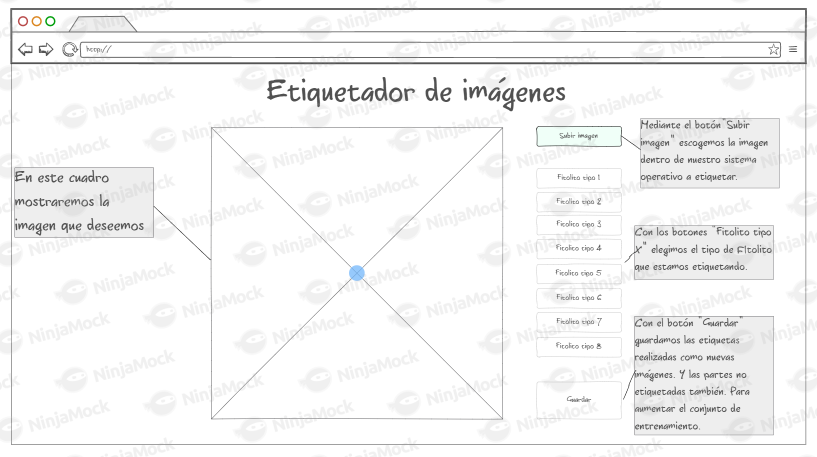
\includegraphics[width=0.99\textwidth]{protototipo_etiquetador_de_imagenes}
\caption{Prototipo del etiquetador de imágenes}
\label{fig:C.5.2}
\end{figure}

El resultado tras la implementación de este producto es el mostrado en la \ref{fig:C.5.3}. Obteniendo una interfaz muy similar a la prototipada en un principio. Pero añadiendo algún elemento más, para facilitar su uso por parte del usuario.

\begin{figure}
\centering
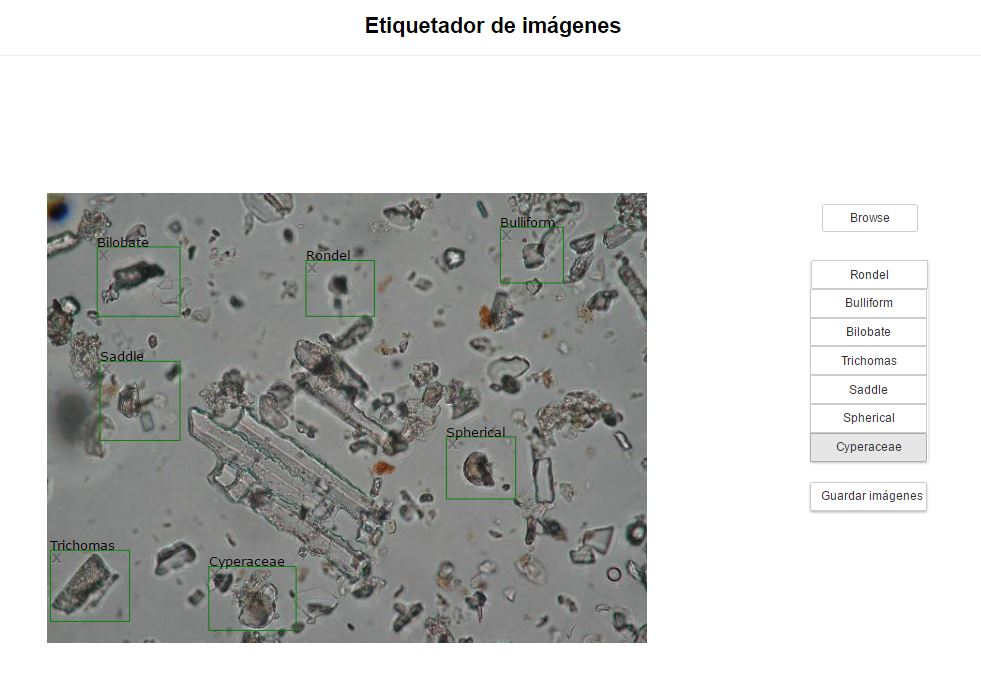
\includegraphics[width=0.99\textwidth]{etiquetador_de_imagenes_v1}
\caption{Etiquetador de imágenes}
\label{fig:C.5.3}
\end{figure}

\subsection{Reconocimiento automático de fitolitos}

La interfaz para el reconocimiento automático de fitolitos consta de un conjunto de \textit{sliders}, los cuales nos permiten cambiar diversos parámetros para experimentar con este y dos botones: botón para subir una imagen y botón para ejecutar el reconocimiento. Véase la figura~\ref{fig:C.5.4}. Cada uno de los botones y \textit{sliders} se encuentran explicados en el manual de usuario~\ref{manuser}.

\begin{figure}
\centering
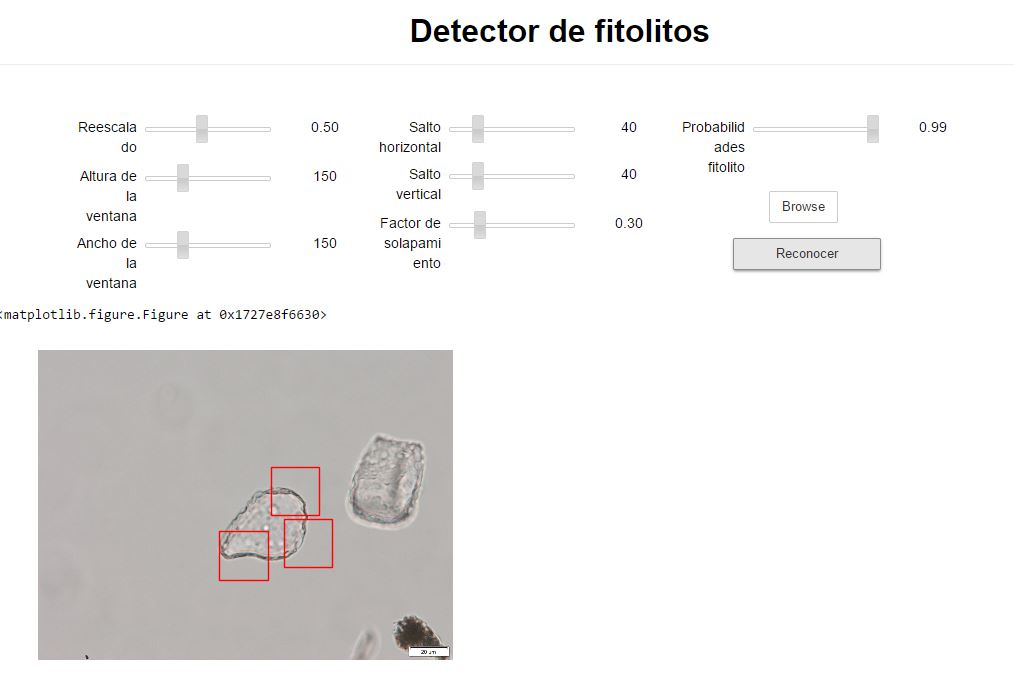
\includegraphics[width=0.99\textwidth]{reconocimiento}
\caption{Reconocimiento automático de fitolitos}
\label{fig:C.5.4}
\end{figure}